\documentclass[a4paper]{article}

\usepackage[T1]{fontenc}
\usepackage[english]{babel}
\usepackage{textcomp}
\usepackage{multirow}
\usepackage{float}
\usepackage{fancyhdr}
\usepackage{pdfpages}
\usepackage{graphicx}
\usepackage{amsmath}

\title{Bayes Classifier and Boosting}
\author{Karl Johan Andreasson <{kalleand@kth.se}> %
\and Christian Wemstad <{wemstad@kth.se}> %
}

\fancyhf{}
\fancyhead[LE,RO]{\slshape \rightmark}
\fancyhead[LO,RE]{\slshape \leftmark}
\fancyfoot[C]{\thepage}

\begin{document}
\thispagestyle{empty}
\maketitle
\thispagestyle{empty}
\pagestyle{empty}
\newpage
\pagestyle{fancy}
\setcounter{page}{1}

\section{Policy Iteration}

\begin{table}[h!]
    \centering
    \begin{tabular}{l|l}
        0 & 1 \\
        1 & 2 \\
        2 & 3 \\
        3 & 7 \\
        4 & 8 \\
        5 & 4 \\
        6 & 7 \\
        7 & 4 \\
        8 & 12 \\
        9 & 13 \\
        10 & 11 \\
        11 & 8 \\
        12 & 13 \\
        13 & 1 \\
        14 & 2 \\
        15 & 14 \\
    \end{tabular}
    \caption{Policy Iteration policy vector with $T = 100$ and $\gamma = 0.5$}
\end{table}

\begin{figure}[h!]
    \centering
    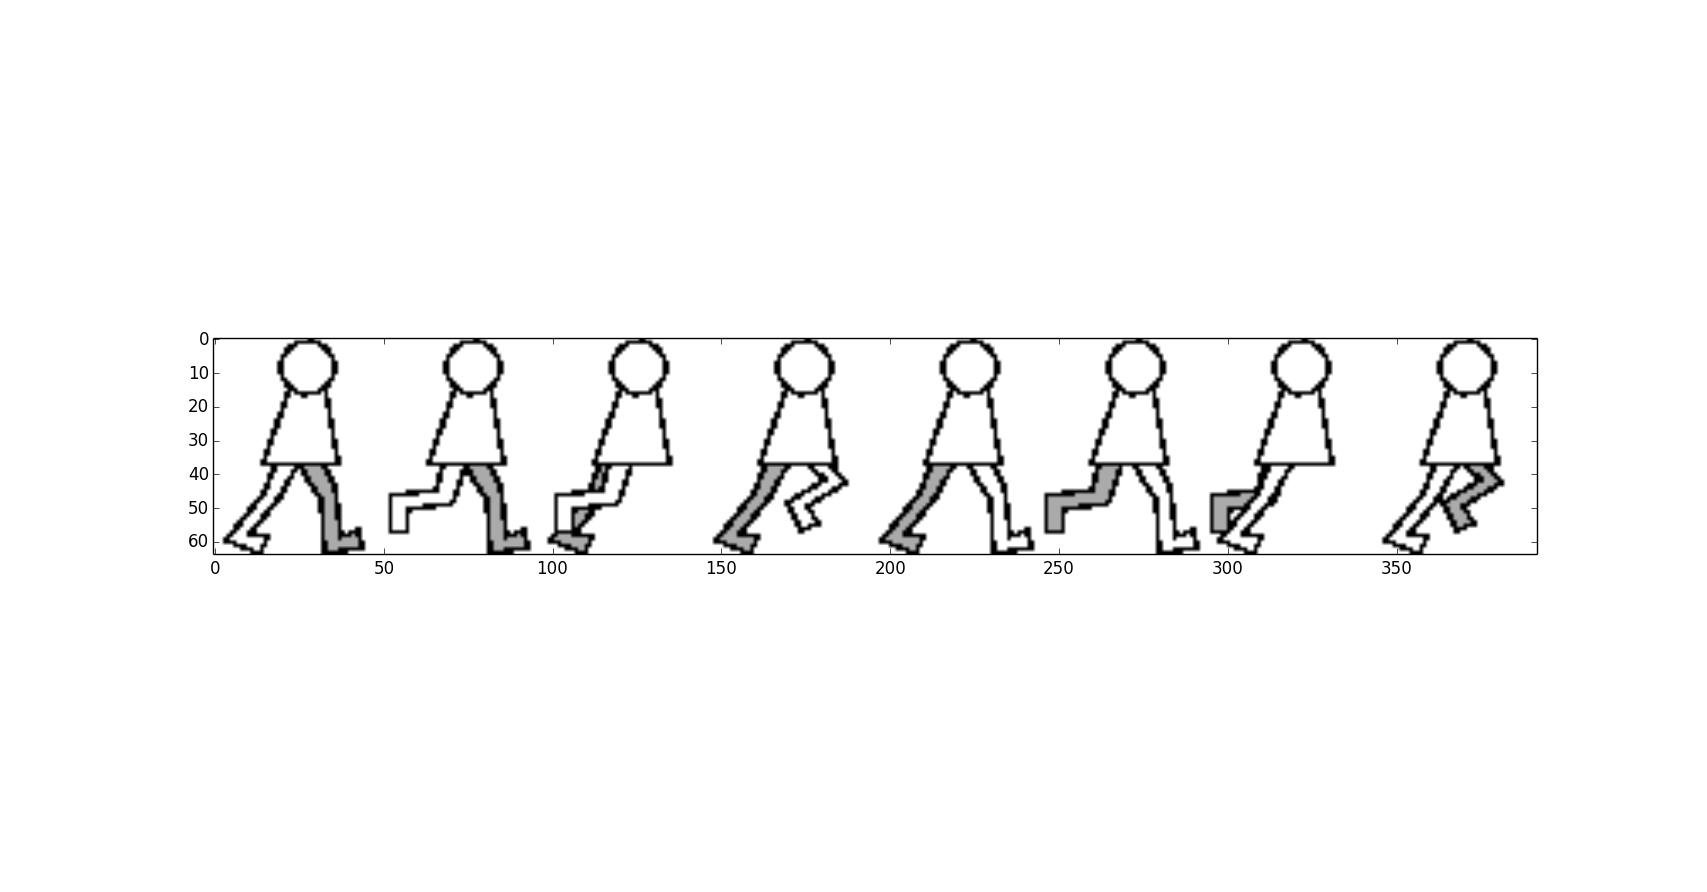
\includegraphics[width=1\textwidth]{qlearning1.png}
    \caption{Policy Iteration loop with $T = 100$ and $\gamma = 0.5$}
\end{figure}

\section{Q-learning}

If you do not use an $\epsilon$ greedy algorithm no new paths will be explored,
meaning that only the seemingly best path in the beginning of the learning
process will ever be taken.

\begin{table}[h!]
\centering
\begin{tabular}{l|l|l|l|l}
    0 & 26.47 & 24.78 & 26.60 & 24.84 \\
    1 & 24.43 & 24.57 & 25.20 & 25.26 \\
    2 & 24.64 & 26.54 & 25.30 & 25.11 \\
    3 & 29.07 & 28.12 & 29.64 & 28.44 \\
    4 & 25.12 & 25.27 & 24.45 & 26.84 \\
    5 & 35.07 & 32.15 & 34.96 & 32.22 \\
    6 & 35.19 & 36.32 & 34.97 & 32.33 \\
    7 & 32.35 & 34.36 & 35.20 & 32.40 \\
    8 & 28.60 & 25.21 & 26.88 & 26.65 \\
    9 & 34.88 & 36.54 & 35.32 & 36.37 \\
    10 & 38.62 & 32.15 & 38.76 & 36.30 \\
    11 & 32.38 & 34.40 & 35.39 & 35.35 \\
    12 & 29.47 & 28.42 & 32.15 & 28.15 \\
    13 & 35.28 & 32.50 & 32.40 & 34.40 \\
    14 & 35.26 & 35.37 & 32.38 & 34.36 \\
    15 & 32.29 & 32.13 & 32.41 & 32.06 \\
\end{tabular}
\caption{Q-learning Q-matrix with $T = 750$, $\gamma = 0.1$, $\epsilon = 0.1$, and $\eta = 0.1$}
\end{table}

Note that we have initiate the Q matrix with the values 100. This is to
enforce that every step gets visited once early.

\begin{figure}[h!]
    \centering
    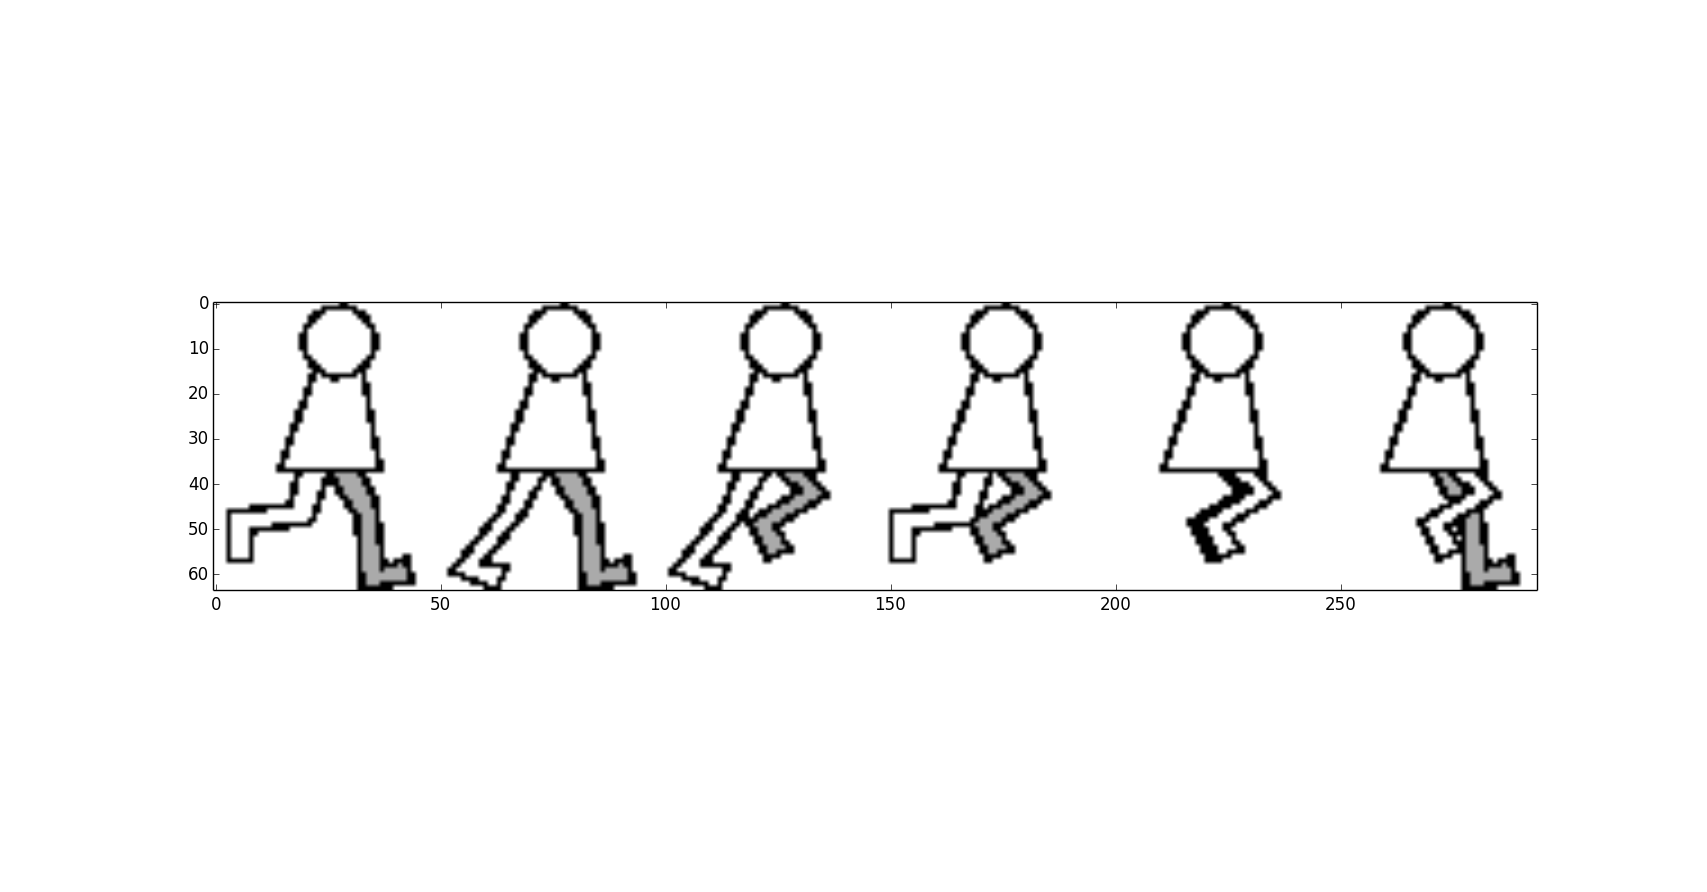
\includegraphics[width=1\textwidth]{qlearning2.png}
    \caption{Q-learning loop with $T = 750$, $\gamma = 0.1$, $\epsilon = 0.1$, and $\eta = 0.1$}
\end{figure}

\begin{table}[h!]
\centering
\begin{tabular}{l|l|l|l|l}
    0 & 3.16 & 0.27 & 3.16 & 2.56 \\ 
    1 & 2.30 & 4.51 & -6.8 & -0.6 \\ 
    2 & 6.44 & 3.28 & -2.1 & 0.24 \\ 
    3 & 4.74 & -6.7 & 9.21 & -1.3 \\ 
    4 & -6.1 & -0.6 & 2.34 & 4.51 \\ 
    5 & 3.51 & 3.10 & 3.49 & 3.26 \\ 
    6 & 9.27 & 2.81 & 8.64 & 6.74 \\ 
    7 & -2.7 & 13.1 & 6.64 & 10.3 \\ 
    8 & -3.2 & 0.46 & 6.44 & 3.23 \\ 
    9 & 7.89 & 8.25 & 9.23 & 7.36 \\ 
    10 & 13.0 & 12.5 & 13.25 & 11.5 \\ 
    11 & 7.21 & 14.5 & 11.62 & 13.0 \\ 
    12 & 9.21 & -1.7 & 4.62 & -6.9 \\ 
    13 & 6.53 & 10.4 & -1.9 & 13.1 \\ 
    14 & 11.7 & 13.3 & 7.74 & 14.5 \\ 
    15 & 10.4 & 3.60 & 10.44 & 6.73 \\
\end{tabular}
\caption{Q-learning Q-matrix with $T = 10,000$, $\gamma = 0.7$, $\epsilon = 0.2$, and $\eta = 0.1$}
\end{table}

\begin{figure}[h!]
    \centering
    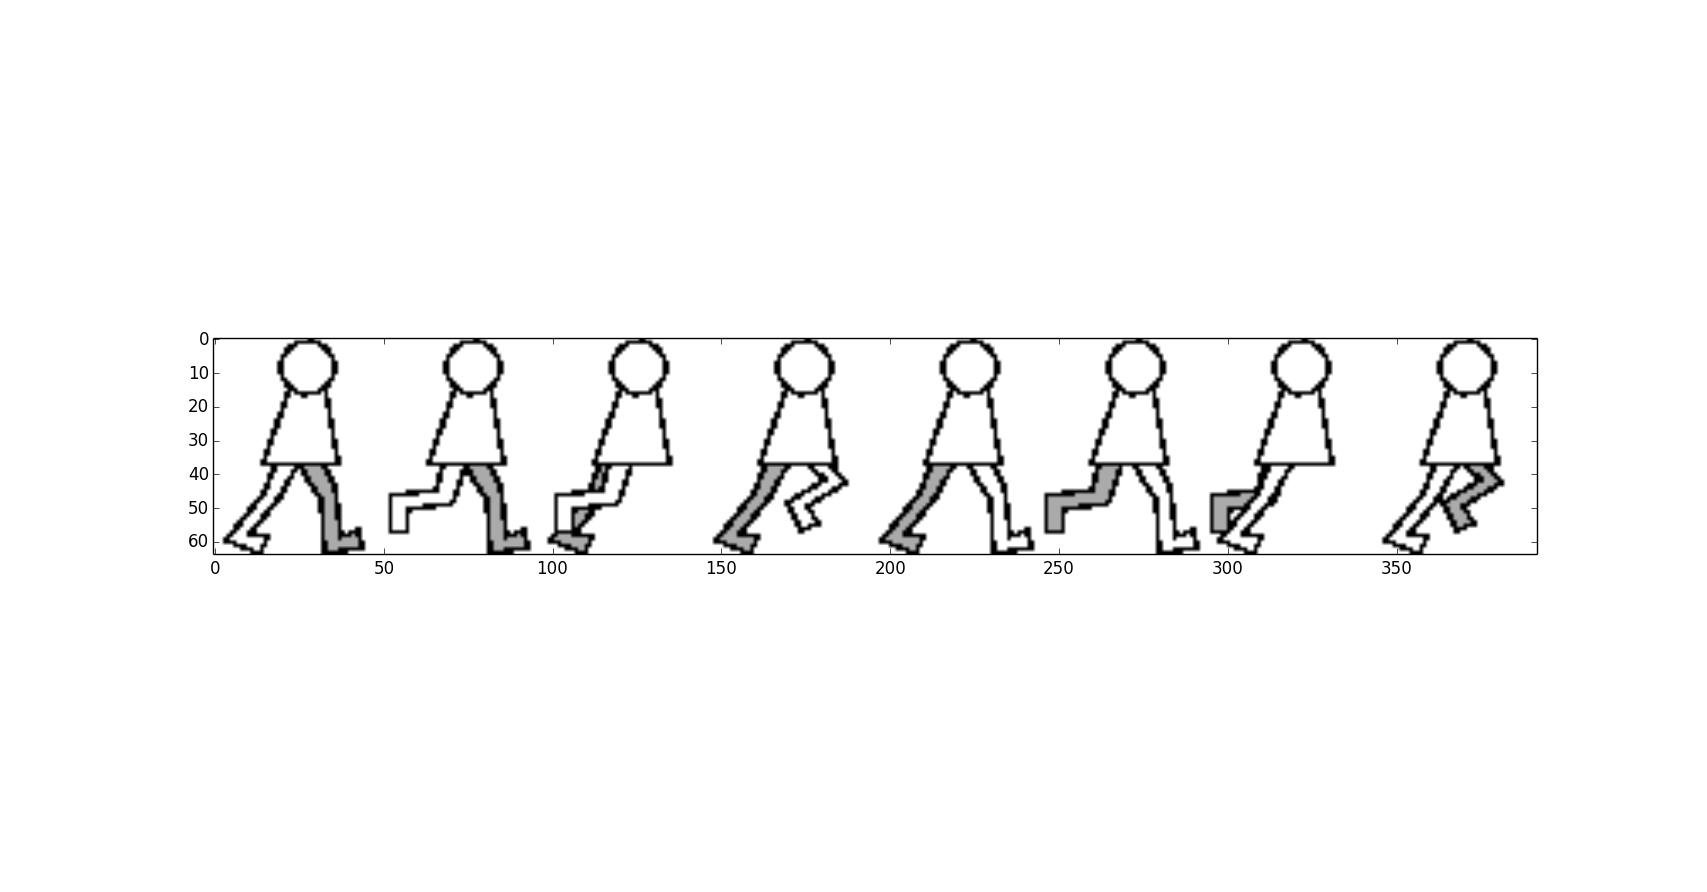
\includegraphics[width=1\textwidth]{qlearning1.png}
    \caption{Q-learning loop with $T = 10,000$, $\gamma = 0.7$, $\epsilon = 0.2$, and $\eta = 0.1$}
\end{figure}

\end{document}
